\documentclass[11pt]{article}
\usepackage[font={scriptsize}]{caption}
\usepackage[utf8]{inputenc}
\usepackage{graphicx}
\usepackage{subfigure}

\title{miniproject}
\author{Zitong Zhao }
\date{December 2022}

\begin{document}
\begin{titlepage}

\includegraphics[scale=0.2]{../data/Imperial - logo.png}
  \begin{center}
    \Huge
        
    \textbf{Selecting the best-fitting model for bacterial cells population growth}
            
    \vspace{1.5cm}
    \Large    
    \textbf{Zitong Zhao}\\
    \vspace{1.5cm}
    
\includegraphics[scale=0.12]{{../data/Shield_IC.png}} \\

    \large
    \vfill       
     Department of Life Sciences, Imperial College London, \\Silwood Park Campus, Ascot SL5 7PY, UK
     \vspace{\baselineskip}
     \\December 2022\\
     \vspace{\baselineskip}
     Word Count: 1623
  \end{center}

\end{titlepage}

\section*{Abstract}
In research on the microbial cells growth, I used two linear models and two non-linear model to fit the data and also for finding the best model of fitting the population data. After data preparation, I transformed and labelled the data. I used OLS to fit quadratic and cubic models and NLLS to fit logistic and Gompartz models. I thoroughly examined how many times AIC, BIC, and \(R^2\) were the best in each subset and eventually decide that the cubic model was the best model in fitting microbial cells population. 

\section{Introduction}
The population grows exponentially while its abundance is low and its resources are not limited (Malthusian principle by \cite{malthus_1989}). As resources become limited, this growth then slows down and eventually stops. There may also be a time lag before population growth really takes off in the first place. We will focus on the growth rate of microbial (especially bacteria).I'll look at how well two phenomenological (cubic and quadratic polynomial) and two mechanistic (logistic and Gompertz (\cite{gompertz1825xxiv}) models fit to growth curves in different bacterial populations.\\
Data fitting is an important form of data processing. When studying two variables, regression analysis can be used to analyse. The number of microbial cells has a certain dependence on the time of growth, and we know that the population can be partially determined by time, but again this relationship is uncertain. So we often use regression models in statistics to find the relationship between the two variables.\\
\newpage
\section{Methods}
\subsection{Data Preparation}
Data on changes in the number of microbial cells were used to explore population growth rates(\cite{roth1962continuity, stannard1985temperature, phillips1987relation, sivonen1990effects, gill1991growth, zwietering1994modeling, bae2014growth, galarz2016predicting, bernhardt2018metabolic, silva2018modelling}). 
These data sets contain measurements of biomass or the number of microbial cells over time. Bacterial growth in these batch cultures follows a set of distinct phases (lag phase, exponential phase, and stable phase).\\
Because the data contain many groups of different species of microbes in different medium, we have to classify the raw data. 
I subdivided the data into 285 groups of different species and medium and labelled them.\\
In general, the range of the original values of the data is very large, so we have to transform the data, using the log () method to compress the data, reduce the skew and make the data closer to the normal distribution, which facilitates the fitting of our model and research.
I tidied up the data by removing data below zero from both the time and population columns, and generate a new column of log bacterial population data.\\
\subsection{Computing tool}
Python is a basic tool for processing the data, specifically using packages Numpy and Pandas to clean and prepare the original data.\\
I used R to fit the linear models and non-linear models, while the linear models are fitted by OLS methods using package minpack.lm.
I visualised the model fitting predict line using package ggplot2 (\cite{ggplot2_citation}).\\
\LaTeX is used for writing up the report, I used this tool for typesetting whole reports and mathematical formulas.\\ 
\subsection{Model fitting}
The Ordinary Least Squares (OLS) method minimises the sum of the squares of the distances from all observations on the scatter plot to the regression line.
The quadratic (Eq. (1)) and cubic (Eq. (2)) models based on OLS was used to fit the microbial cells population,
and these are phenomenological models which commonly used for seeking the best describe the data.
	\begin{equation}
		N_t = at^2 + bt + c
	\end{equation}
	
	\begin{equation}
		N_t = at^3 + bt^2 + ct + d
	\end{equation}
When a trait determines individual fitness, changes in this functional trait can lead to changes in population growth rate and persistence. 
In data fitting and predicting, I used Non-Linear Least Squares (NLLS) to fit the logistic (Eq. (3)) and Gompertz (Eq. (4)) these mechanistic models.

 
	\begin{equation}
		N_t = \frac{N_0Ke^{rt}}{K + N_0(e^{rt} - 1)}
	\end{equation}
	
	\begin{equation}
		log(N_t) = N_0 + (N_{max} - N_0)e^{-e^{r_{max}exp(1)\frac{t_{lag}-t}{(N_{max}-N_0)log(10)}+1}}
	\end{equation}
	$t$ - time; $N_t$ - population size at time t; $K$ - carrying capacity; $r$ - highest rate of population growth reached; $t_{lag}$ - delay until population growth, or x-axis intercept of the tangent $r$

\section{Results}
In performing the model fit, I subtracted data groups with fewer than five variables, and only 275 data groups were fitted out of 285 sets of data. For these data groups, I fitted every subset by using a 'for' loop. All the data set can be fitted by quadratic and cubic models. However, for non-linear models, we need to find the value of functional traits in each set of data, otherwise the fitted model will not be successfully found. 
Unlike the Logistic model fit to the original non-transformed data, in Gompartz model, it is in the log scale and designed to be fitted to log-transformed data. 
I used a number of random numbers as traits and tried them one by one until I could fit the Gompartz model. For comparison purposes, I use log on the microbial cell population data, where let those phenomenological models to fit the log population. In processing on logistic model, I log the Equation 3 to fit the transformed data; but I also fitted the non-transformed data to give additional check on the goodness of fit on microbial population by logistic model.\\
\begin{figure}[!h]
  \centering
  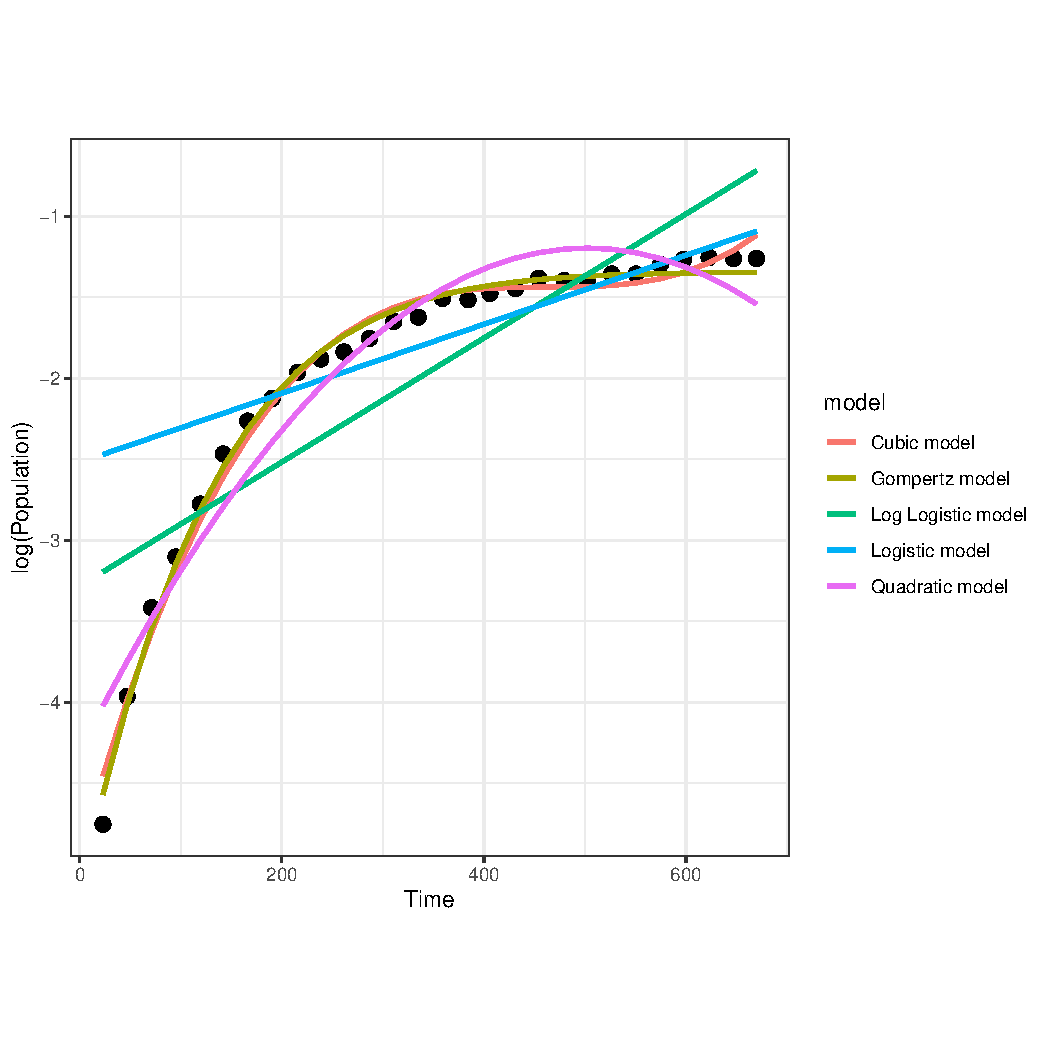
\includegraphics[scale=0.5]{{../data/p1.pdf}}
  \caption{{Population growth curves from the first subset fitted by quadratic, cubic, logistic, Gompertz and log logistic models,The blue line: the predict line which use the results data from non-transformed population fitted by original logistic model.The green line:the predict line which use the results data from transformed population fitted by log logistic model.}}
  \label{fig}
\end{figure}
\newpage
In model fitting, there are lots of commonly used model selection methods. I chose \(R^2\), Akaike information criterion (AIC) and Bayesian Information Criterion (BIC).
R-squared is generally used in regression models to assess the degree of conformity between predicted and actual values. It calculates on rate of unexplained variable, which focus on the degree of fit.The AIC and BIC weigh the complexity of the estimated model against the goodness of the model's fit to the data, with the BIC taking into account the large number of samples to prevent excessive model complexity caused by high model accuracy, while the AIC is for forecasting purposes.\\
Based on my efforts above, I have fitted the four linear and non-linear models and visualised them. The first group contains 28 data which form a typical growth curve shown on figure 1. \\
It shows that the cubic and Gompartz models fit very well of the data, and the quadratic model fits slightly less well, whereas the logistic model is looked like unfitted. We knew that before we fitted the model that the logistic model would have some bias for log data. According to table 1, it is the model selection results from those models fitting on the first subset. The last row of logistic model is a fit to the non-transformed data and can be shown it is good fit from the AIC and BIC. The first four rows are the results of the log population data fit model, which allows us to compare the fit of the various models. Those methods shows that the cubic and Gompartz models can fit the data well than others, it is constant with the graph we drew.
\begin{table}[!h]
    \centering
    \begin{tabular}{c|c|c|c}
    \hline
        Models&\(R^2\)&AIC&BIC\\
        \hline
        quadratic & 0.935&3.585&8.914 \\
         cubic& 0.988&-40.79&-34.129\\
         log logistic&0.715&44.978&50.307\\
         Gompartz&0.993&-58.003&-51.342\\
         logistic&0.832&-98.55&-93.22\\
         \hline
         
    \end{tabular}
    \caption{Model selection methods of the first subset}
    \label{tab:my_label}
\end{table}

Then I have selected two more typical data sets 118 and 261 (figure 2). The fit of the individual models for both sets of data is good, reflecting the fact that the models are able to fit some of the data observations. The models I have chosen are all capable of fitting microbial cell population data and prediction.\\
  \begin{figure}[!h]
    \centering
        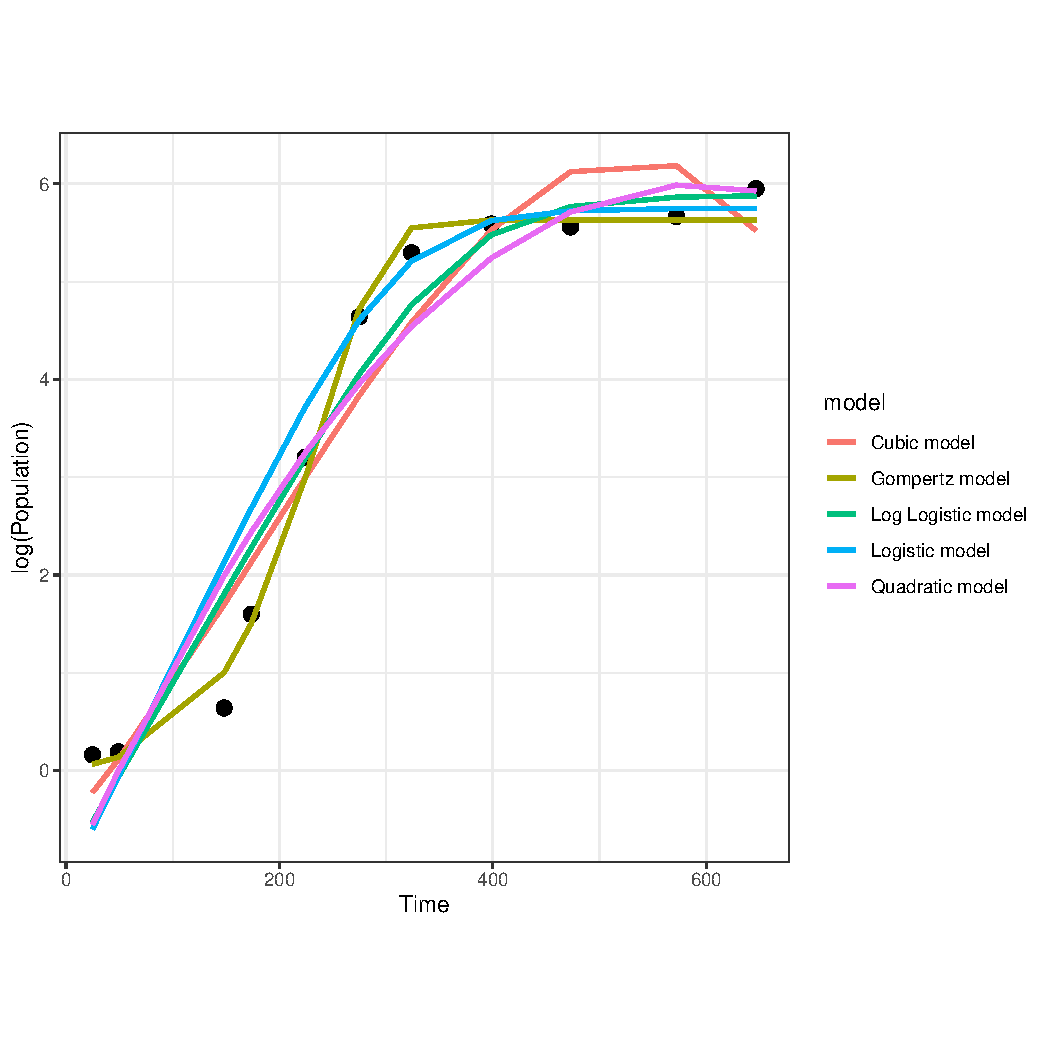
\includegraphics[scale=0.3]{{../data/p118.pdf}}
        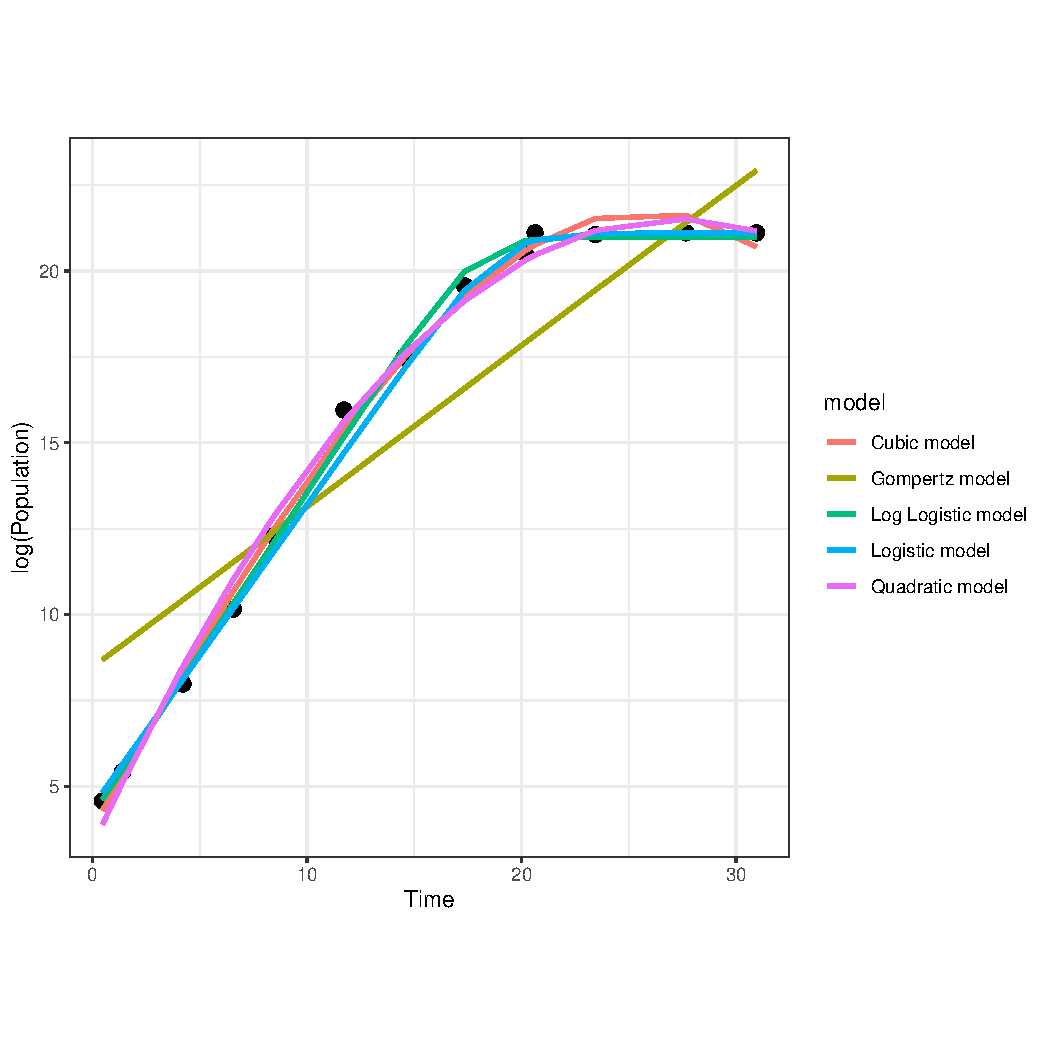
\includegraphics[scale=0.3]{{../data/p261.pdf}}
    \caption{{Population growth curves from the 118 (left) and 261 (right) subset fitted by quadratic, cubic, logistic, Gompertz and log logistic models.}}
    \label{fig}
  \end{figure}
\newpage
To choosing the best fitting model, I have recorded the best \(R^2\), AIC, and BIC of each subset and count the times (Figure 3).\\
  \begin{figure}[!h]
    \centering
    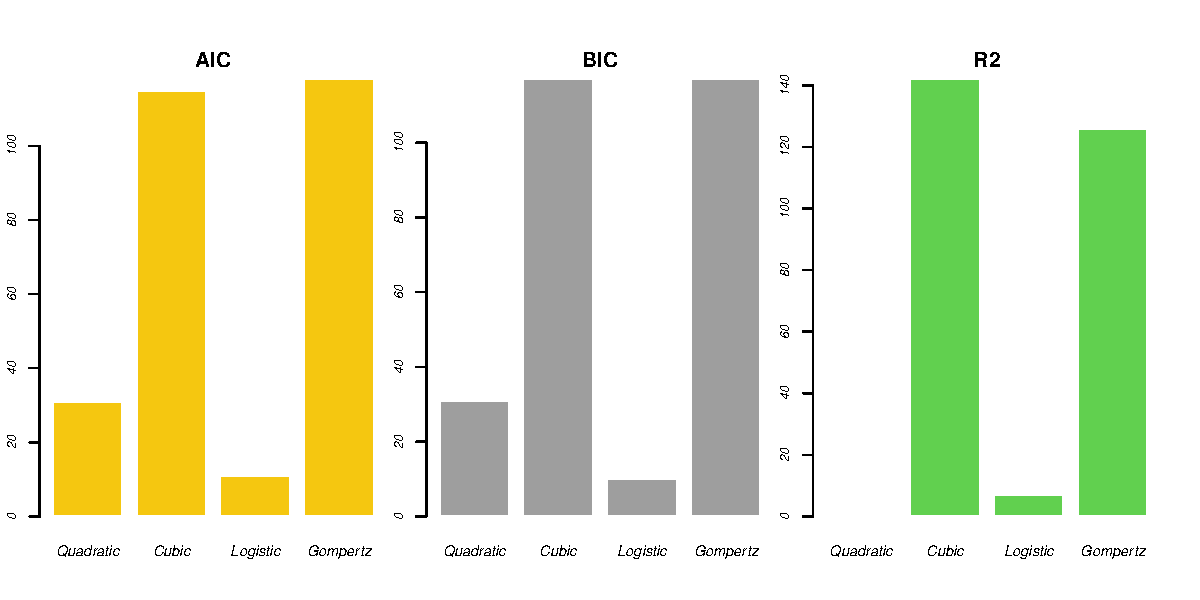
\includegraphics[scale=0.6]{{../data/bestfit.pdf}}
    \caption{Best model choosing by model selection methods}
    \label{fig}
  \end{figure}
For the three model selecting methods, cubic model performed the best of AIC, BIC, \(R^2\), at more than 120, Gompartz model also performed well at more than 100, whereas logistic model is less than 10 of all methods.
In calculating \(R^2\), quadratic model had never become the best model in these 275 data sets, it means that the population growth is not that accurate to be fitted or predicted by using the simply quadratic model.
From the statistical results, the cubic model is the best one to fit the microbial cells population, followed by Gompertz model, these two models fit almost all subsets of the data very well.


\newpage
\newpage
\section{Discussion}
I fitted the quadratic and cubic model using the OLS method and fitted the logistic and Gompartz model using NLLS method. Then I chose the cubic model is the best model to fit the microbial cells population log data according to the model selection methods. Throughout the study I have fitted all 275 subsets of the model and visualised them all to give a more visual representation of how well the model fits. In choosing the best model, I calculated the number of times AIC BIC and \(R^2\) got the best in each subset, and finally, very rigorously, I got cubic as the best model.\\
In dealing with logistic model, I used the whole formula in log to gain a log logistic model, and then compared to other models, however, such an approach may also have led to a significant bias in the fit of the model, resulting in a low score for the logistic model.
Although I removed a subset of less than five data, there were still many subsets with very little data, which led to an easy fit, so that the resulting best-fit model was not very informative.\\
I researched on the microbial population growth with time, and found the cubic model is the best fitting model. The population growth is not only affected by time, but it also affects by temperature and other factor. In this report, I only consider the time as the reason of population change for fitting the linear and non-linear model. For different temperature, species and medium, I only classify them rather than comparing each group, therefore, the population growth under different living conditions has not been explored yet. However, we can identify the model with the highest overall score to fit the growth of microbes under different conditions. There are many other factors that affect the survival of microbial cells in reality that are not affected in the laboratory, and there are still differences between the data obtained and the real population, which could be the focus of my research in the future as I continue to investigate.

\bibliographystyle{plain}
\bibliography{report}
\end{document}